\documentclass[11pt]{article}
\usepackage[english]{babel}
\usepackage[utf8]{inputenc}
\usepackage{amsmath}
\usepackage{graphicx}
\usepackage{fullpage}
\usepackage{setspace}
\usepackage{color}
\usepackage[font=footnotesize]{subcaption}
\usepackage{natbib}
\usepackage[font=footnotesize]{caption}
\usepackage{authblk}
\usepackage[margin=1.0in]{geometry}
\usepackage{mathtools}
\usepackage{graphicx}
\graphicspath{ {./plots/} }

\begin{document}


\title{Programming task 1 and 2}

\author{Kartheek Minnikanti}

\maketitle

\section{Heat diffusion}

Given square domain of [0,1] x [0,1]
\\*Initial condition: at t=0
\\*	inside the circle with radius $\sqrt{0.2}$ and center at (0.5,0.5) , T= 40 C
\\*	inside the square and outside the circle, T= 20C
\\*Boundary Condition:  Boundary at 20 C
Discretization scheme - finite difference method. For this problem central difference forward time is used. Scalar Temperature  field for a time step is calculated from its previous time step alone. In simple words, for this solver Explicit method is used. Time step chosen is '0.05 sec' for stability. Domain discretization is done using square elements having uniform mesh over the given square plate. Solution with different mesh sizes is also compared in the result.
\\*\textbf{Energy conservation equation}
\\*Assumptions: No advection affects. No sources/sinks. Isotropic thermal diffusivity - $\alpha =k / c \rho $ (where 'k' is thermal conductivity, 'c' is heat capacity at constant pressure and $\rho$ is density). Since, in problem no material or transport properties are mentioned, assemed for $\alpha$ value as 0.00001 $m^2$/second (it is closer to value of Al alloys). in z-direction, no changes to temperature values)
\\* For a 2D problem (considering above assumptions),
\begin{equation}
\frac{\partial T}{\partial t} = \alpha (\frac{\partial^2 T}{\partial x^2}+\frac{\partial^2 T}{\partial y^2})
\end{equation}
Considering square mesh in 2D, final discretization equation for $(n+1)^{th}$ iteration from $n^{th}$ iteration (i,j are x,y coodinates) is 

\begin{equation}
T_{i,j}^{n+1} = T_{i,j}^n + \frac{\delta t\alpha}{(\delta x)^2} (T_{i+1,j}^n+T_{i-1,j}^n+T_{i,j+1}^n+T_{i,j-1}^n-4T_{i,j}^n)
\end{equation}
\\*Code is written using c++ and it takes 3 inputs- n(for domain discretization),dt(time step) and t(final time). It writes the required output to a text file. Below plots compare temperature profile at 3 mesh sizes (50x50,100x100,200x200) in increasing order. 
\\*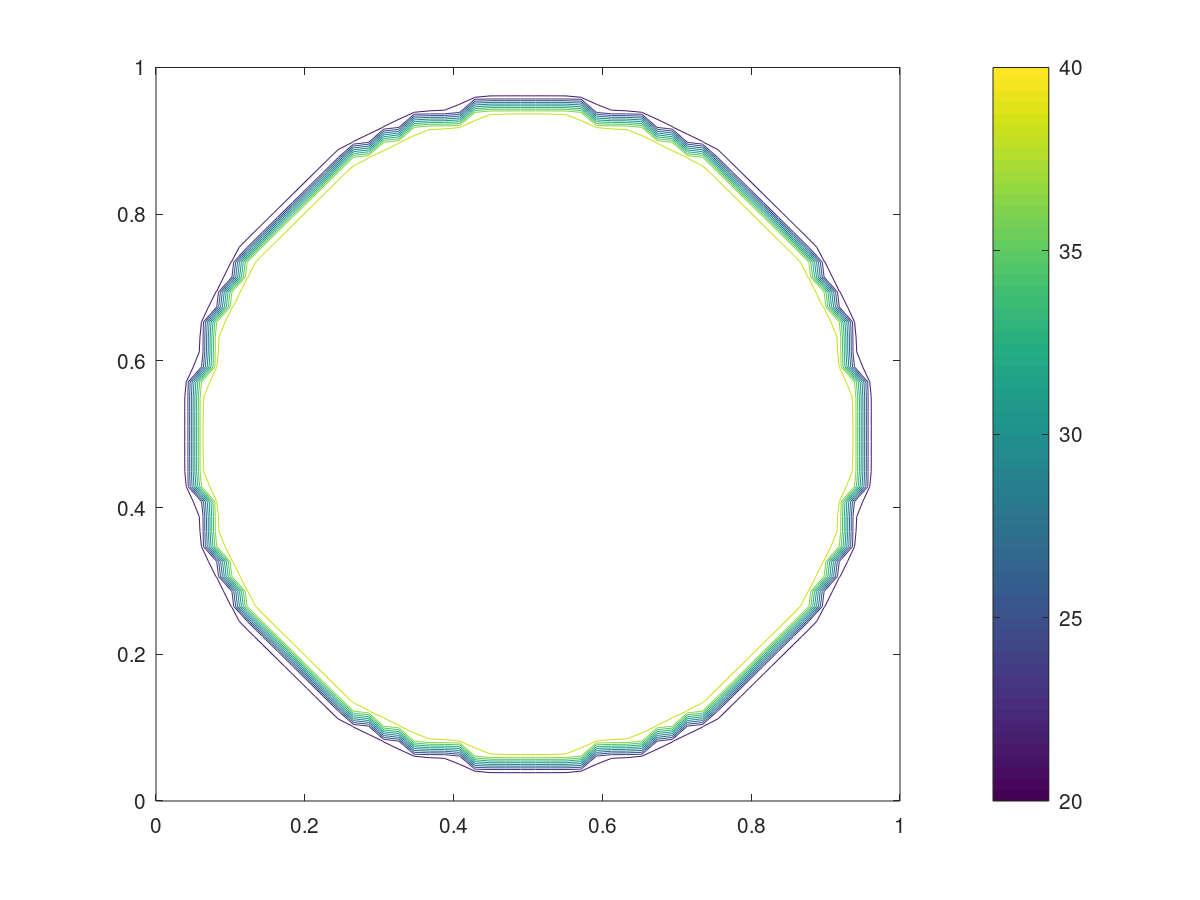
\includegraphics[scale=0.11]{5sec50.png}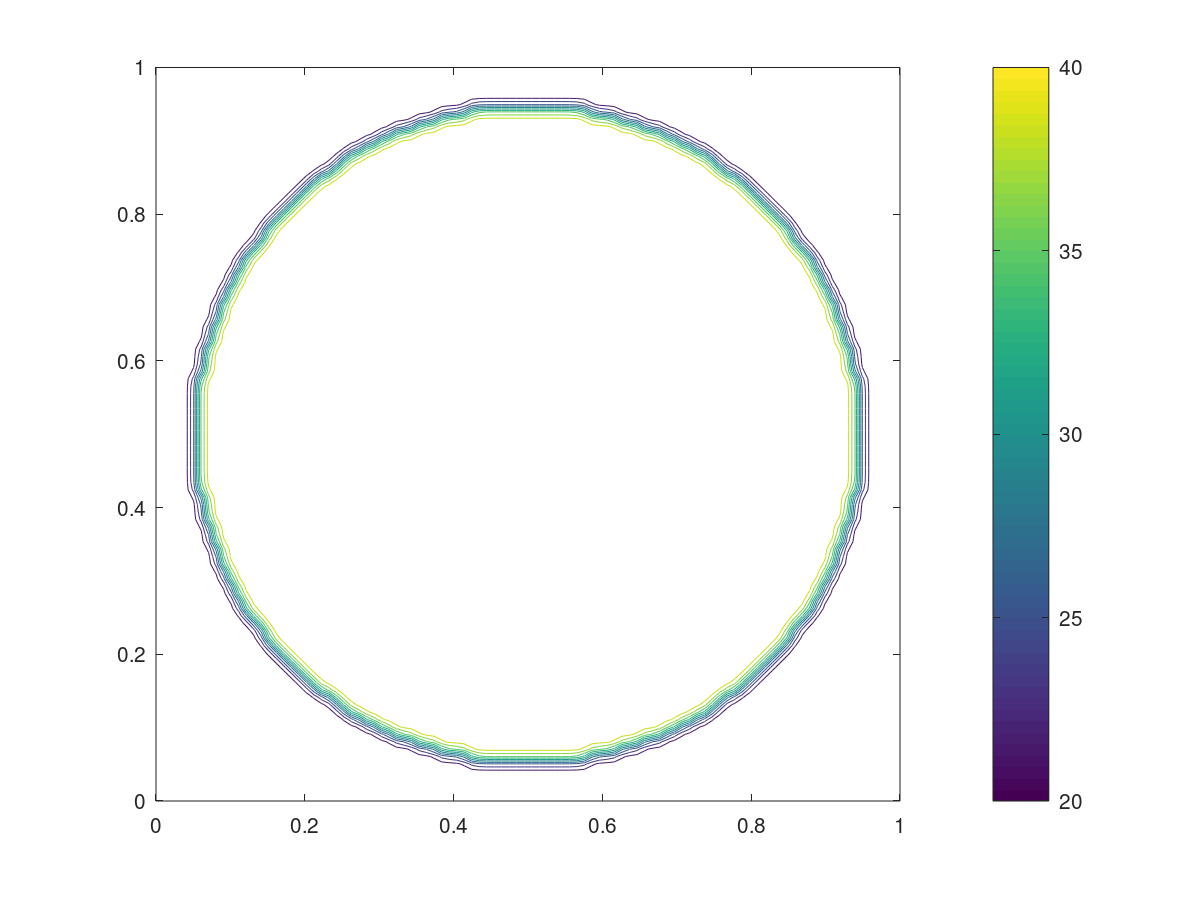
\includegraphics[scale=0.11]{5sec.png}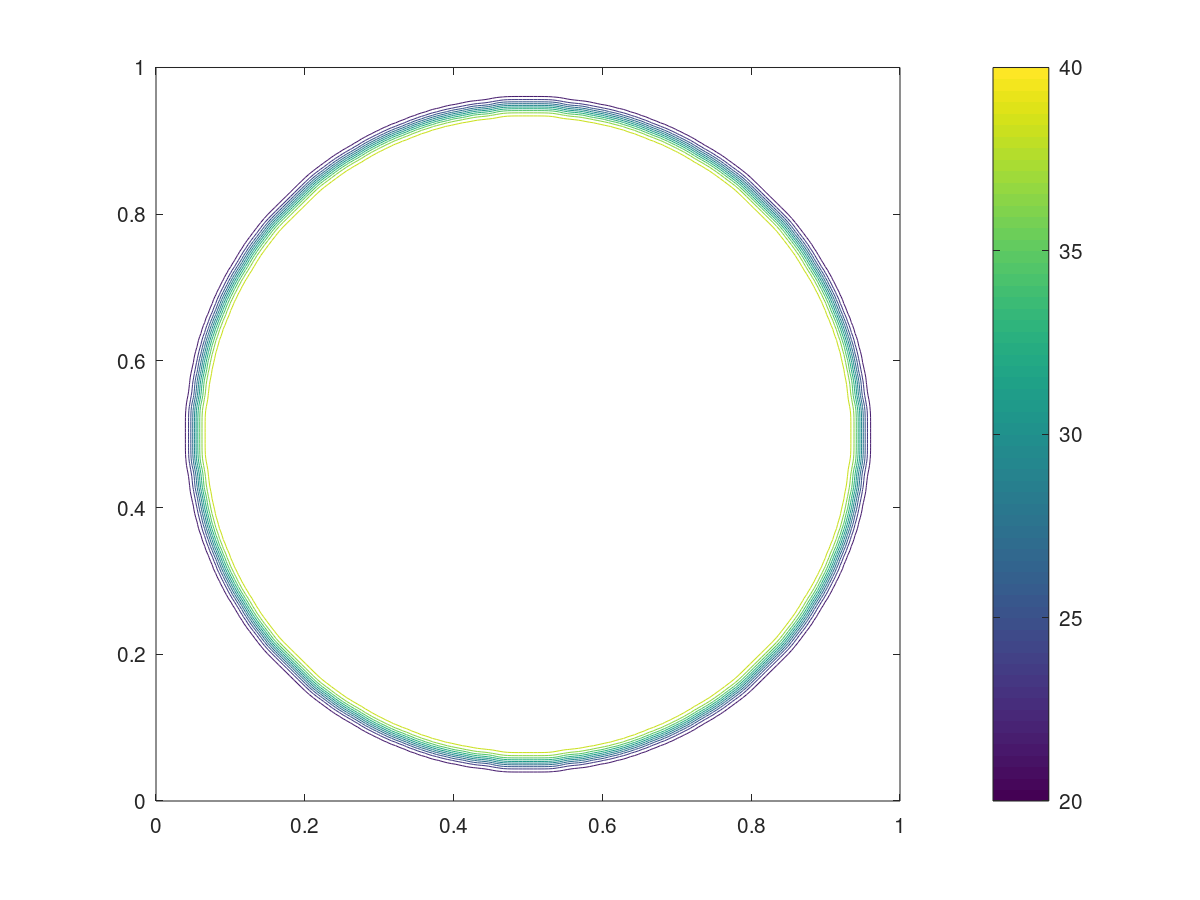
\includegraphics[scale=0.11]{5sec200.png}
\\*Chosen mesh size is 100x100 and the results at different time steps are plotted at 0s, \\*5s,20s,50s,200s,500s,2000s,7200s. All the plots in the increasing order of time are,
\\*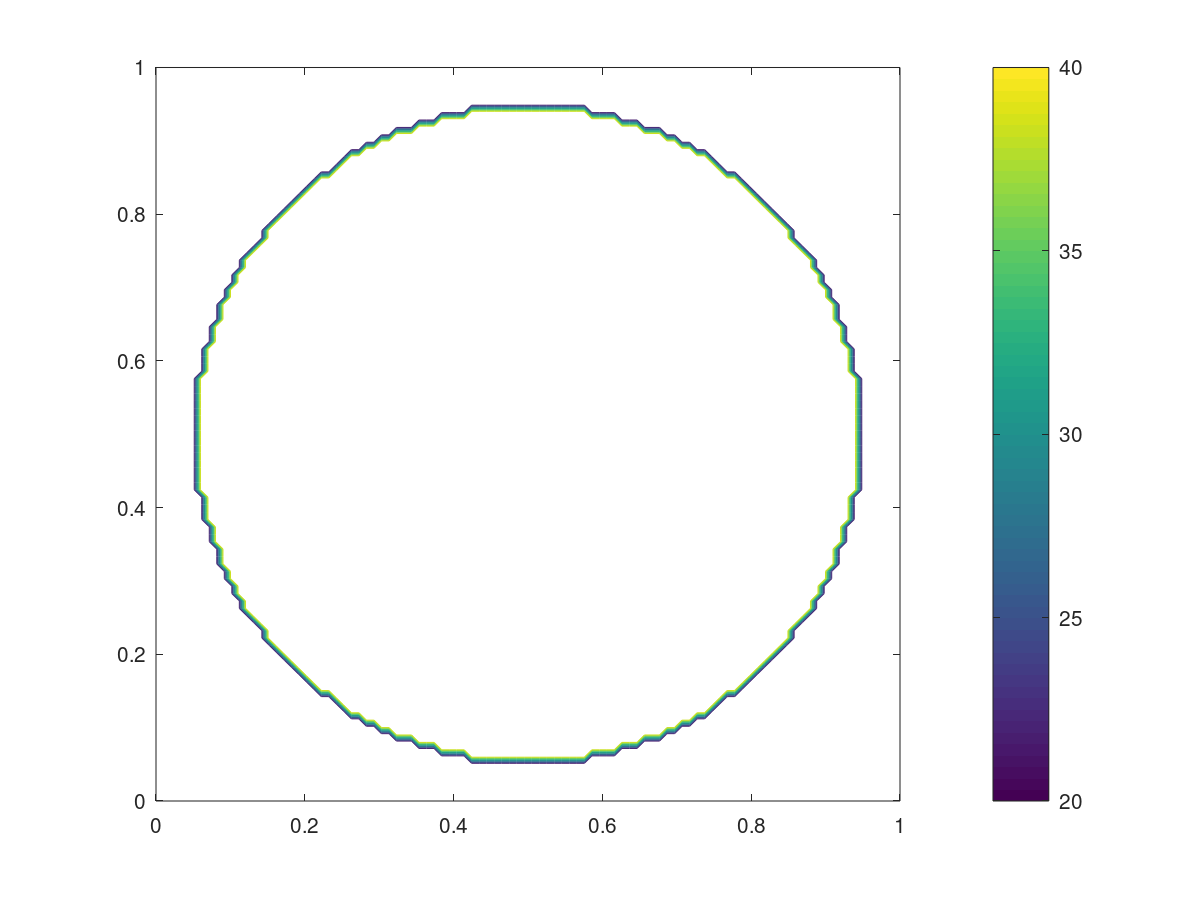
\includegraphics[scale=0.11]{0sec.png}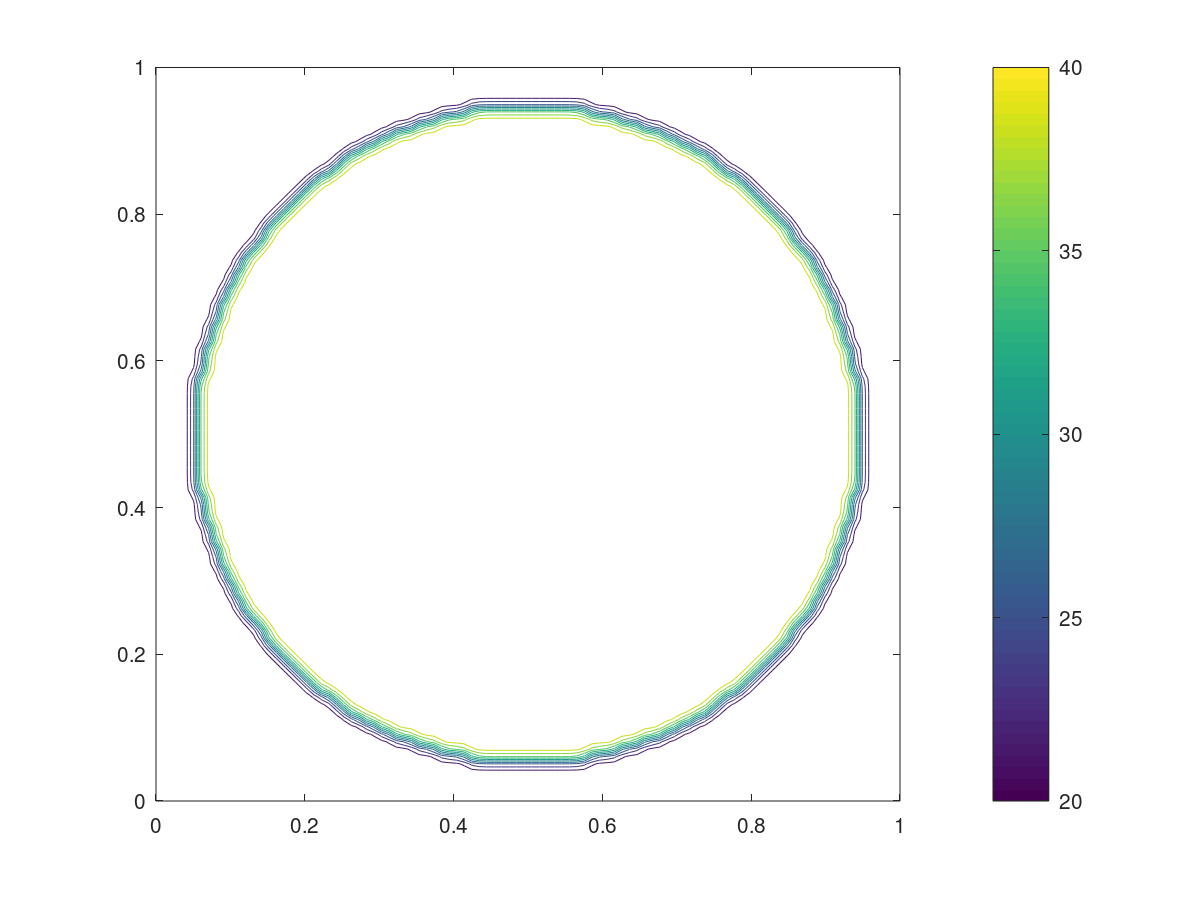
\includegraphics[scale=0.11]{5sec.png}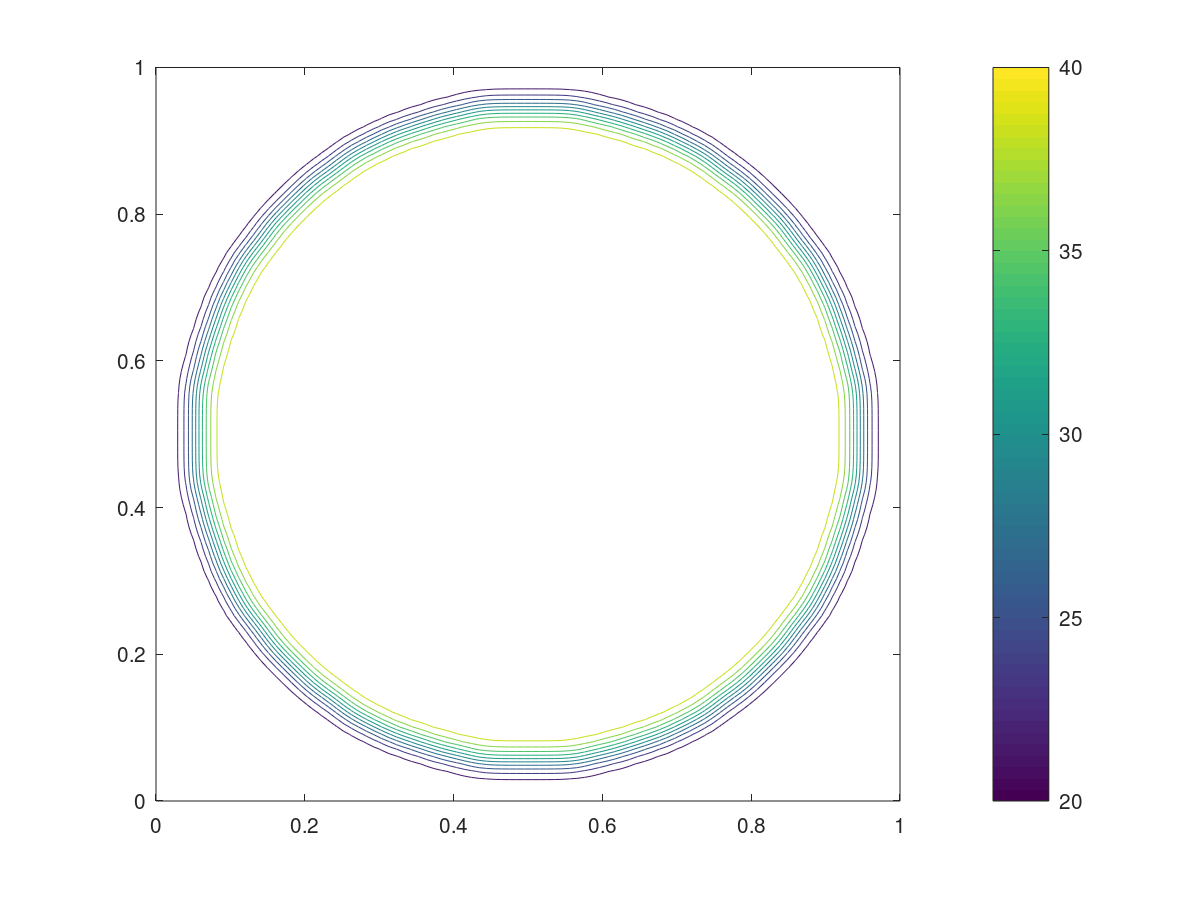
\includegraphics[scale=0.11]{20sec.png}\\*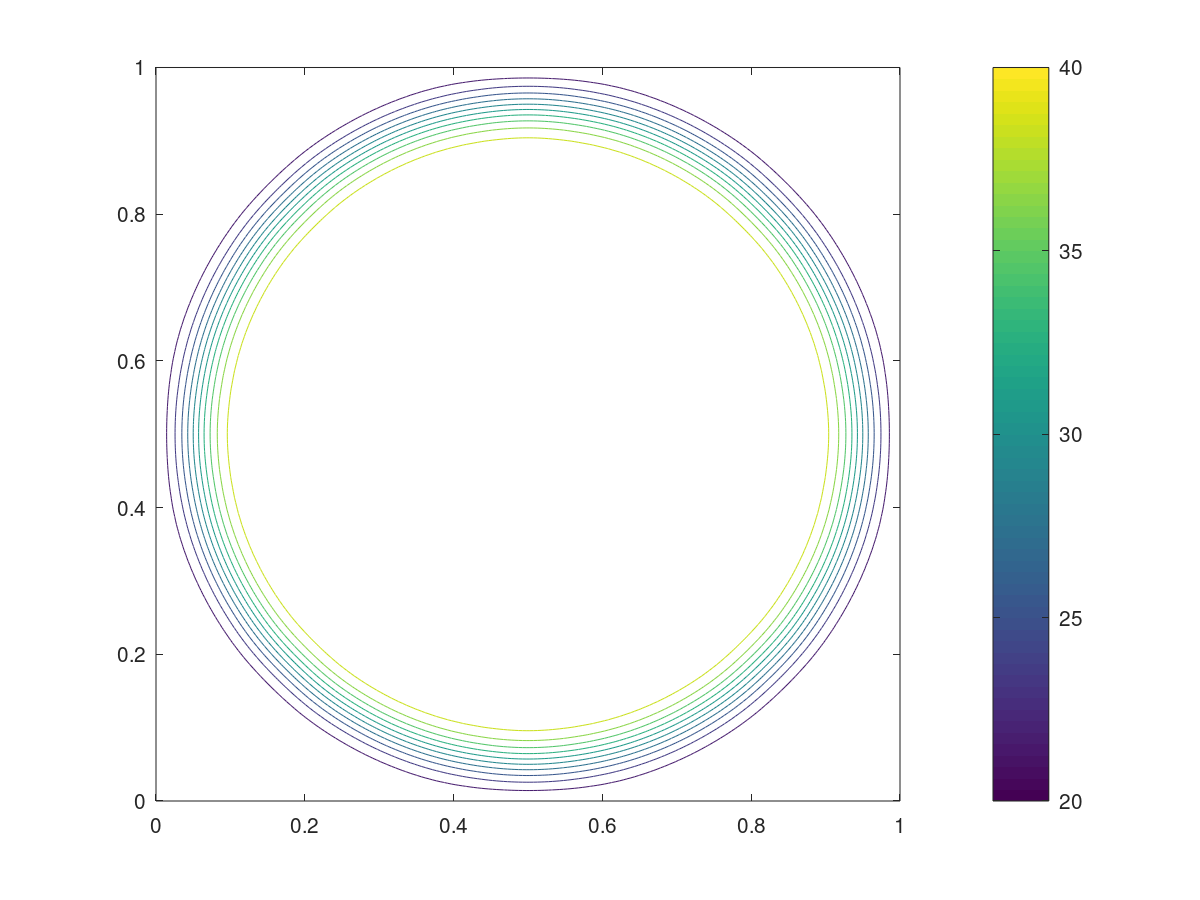
\includegraphics[scale=0.11]{50sec.png}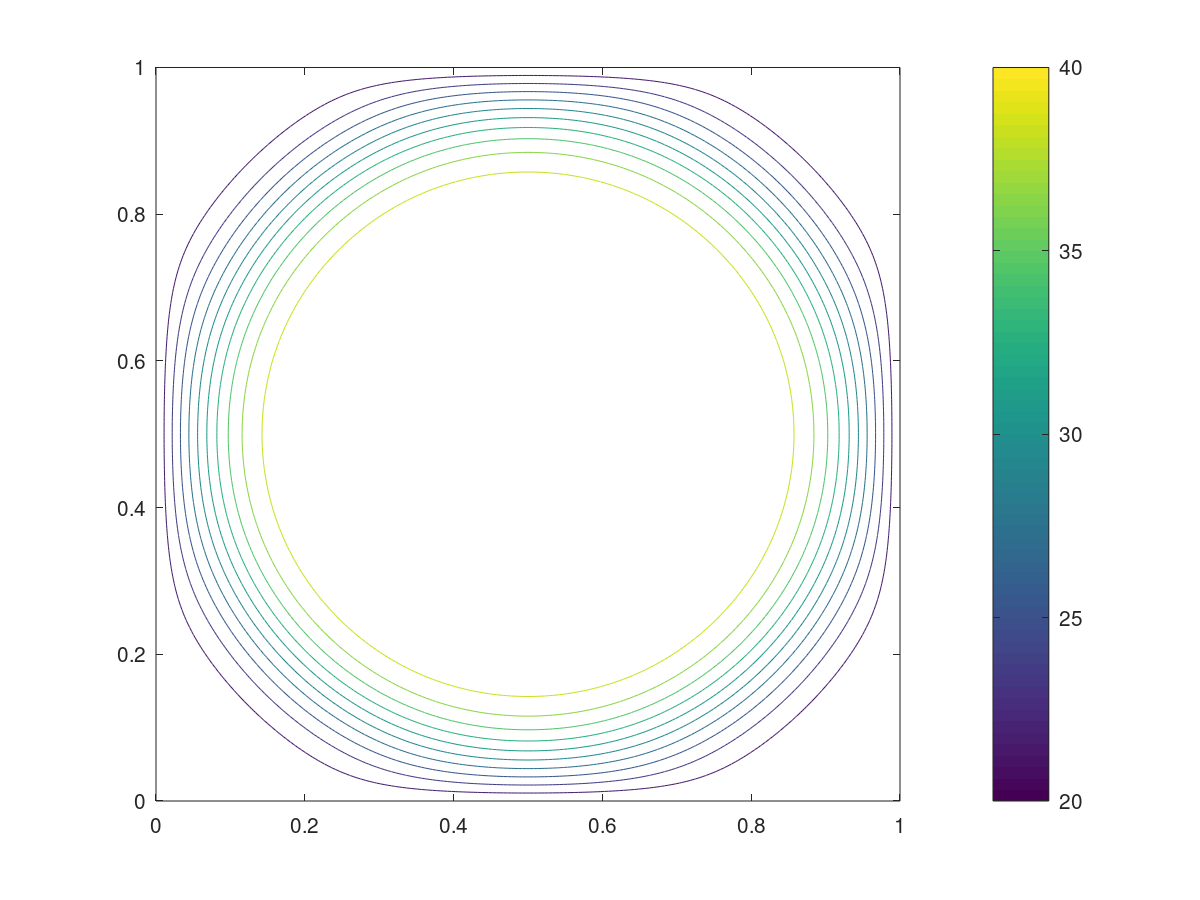
\includegraphics[scale=0.11]{200sec.png}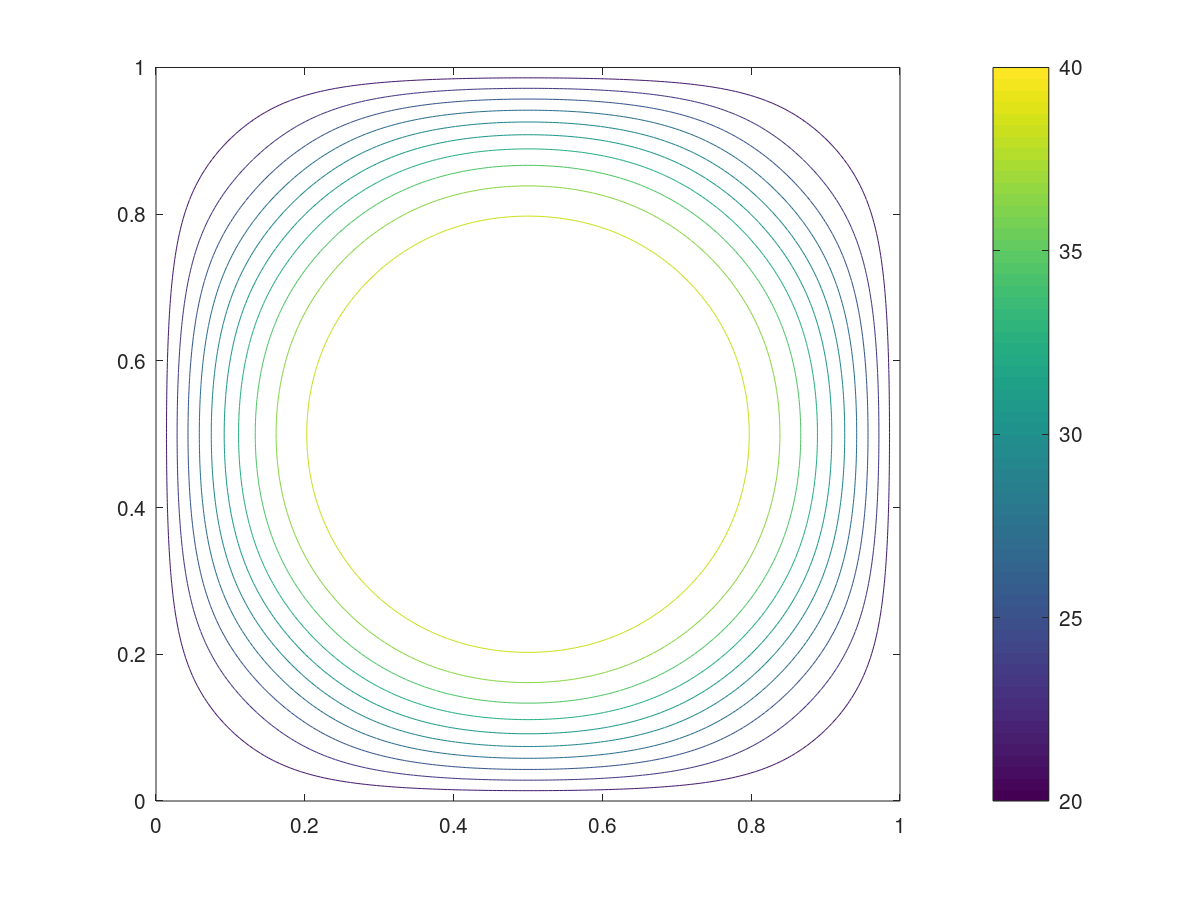
\includegraphics[scale=0.11]{500sec.png}\\*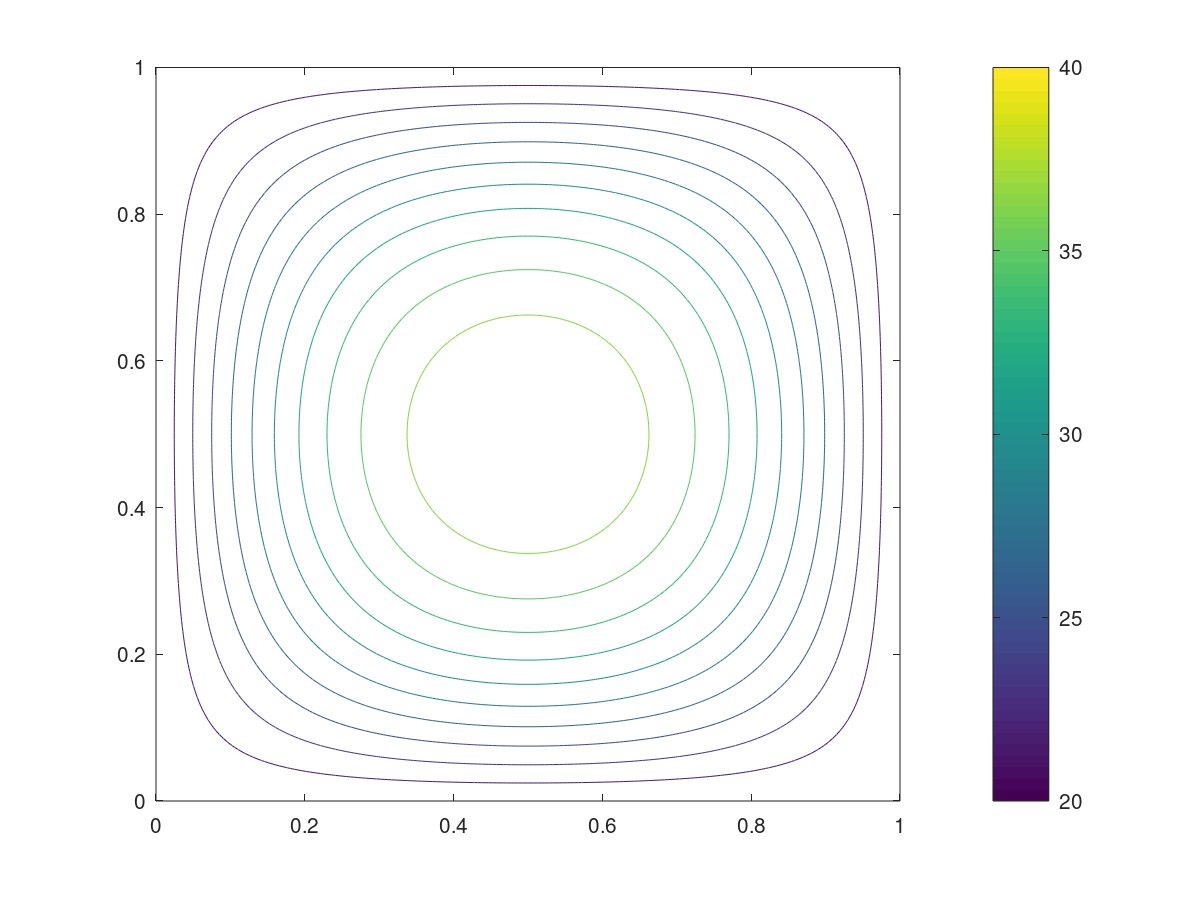
\includegraphics[scale=0.11]{2000sec.png}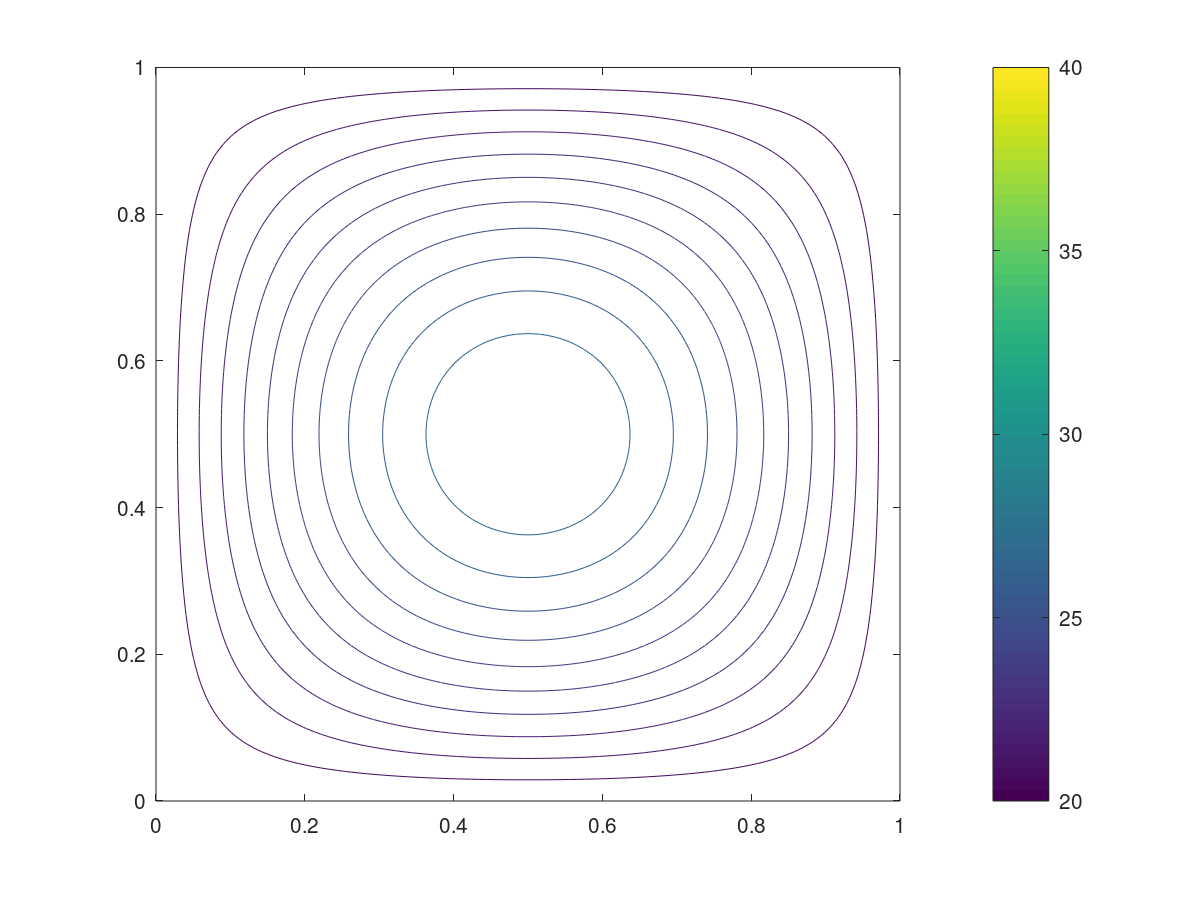
\includegraphics[scale=0.11]{7200sec.png}
\\*\textbf{Comments}: Since all the bounadaries are maintained at a constant temperature of 20 C, energy transport will occur and eventually a constant sclare field same as the tempearature at boundaries is expected and same is observed in this simulation. 

\section{Monte carlo simulation}
For given ODEs, initial condition mentioned is (1,1,1) at '0'. Explicit RK-4 scheme to solve the given coupled systme is given below. Since all derivatives are not dependent 't', its not considered (because it will yield zero values).  
\begin{equation}
\frac{dx}{dt} =f_x(x,y,z)=10(y-x)
\end{equation}
\begin{equation}
\frac{dy}{dt} =f_y(x,y,z)=x(28-z)-y
\end{equation}
\begin{equation}
\frac{dz}{dt} =f_z(x,y,z)=xy-\frac{8}{3}z
\end{equation}
\\* for  $(i+1)^{th}$ step using $(i)^{th}$ step,
\begin{equation}
x_{i+1}=x_i+\frac{1}{6}(k_1+2k_2+2k_3+k_4)
\end{equation}
\begin{equation}
y_{i+1}=y_i+\frac{1}{6}(l_1+2l_2+2l_3+l_4)
\end{equation}
\begin{equation}
z_{i+1}=z_i+\frac{1}{6}(m_1+2m_2+2m_3+m_4)
\end{equation}
'h' is the step size and $\phi$=(k,l,m),
$k_1=hf(x_i,y_i,z_i),
k_2=hf(x_i+0.5k_1,y_i+0.5l_1,z_i+0.5m_1),
k_3=hf(x_i+0.5k_2,y_i+0.5l_2,z_i+0.5m_2),
k_4=hf(x_i+k_3,y_i+l_3,z_i+m_3)$
\\For IVP with initial value of (x,y,z)  is a joint Gaussian with mean (1,1,1) and covariance of identity matrix. Same is simulated using monte-carlo for the given coupled ODEs. Pairwise joint PDFs are plotted (in order xy,yz,zx) in histograms below at t=0,0.2,0.5,1.0 ( in the same order)
\\*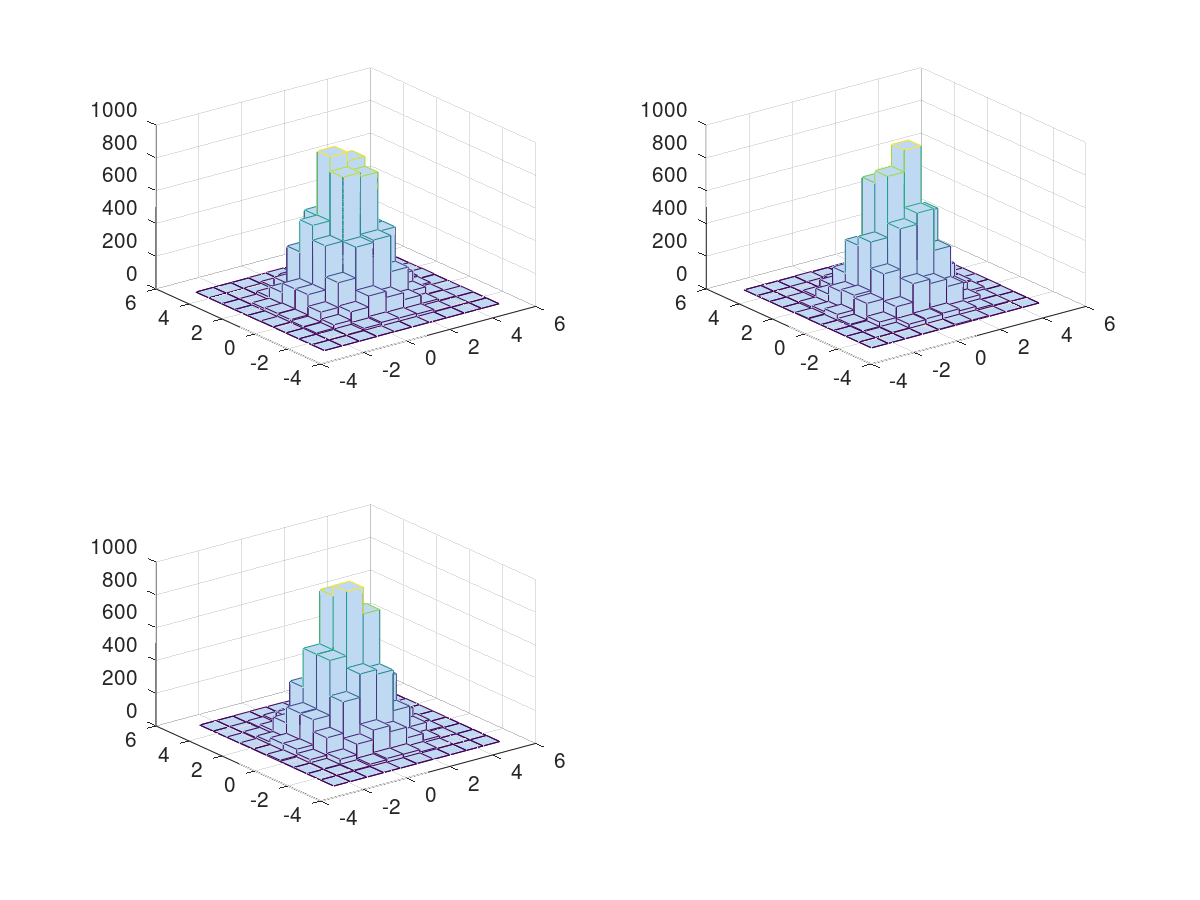
\includegraphics[scale=0.2]{t_0.0.png}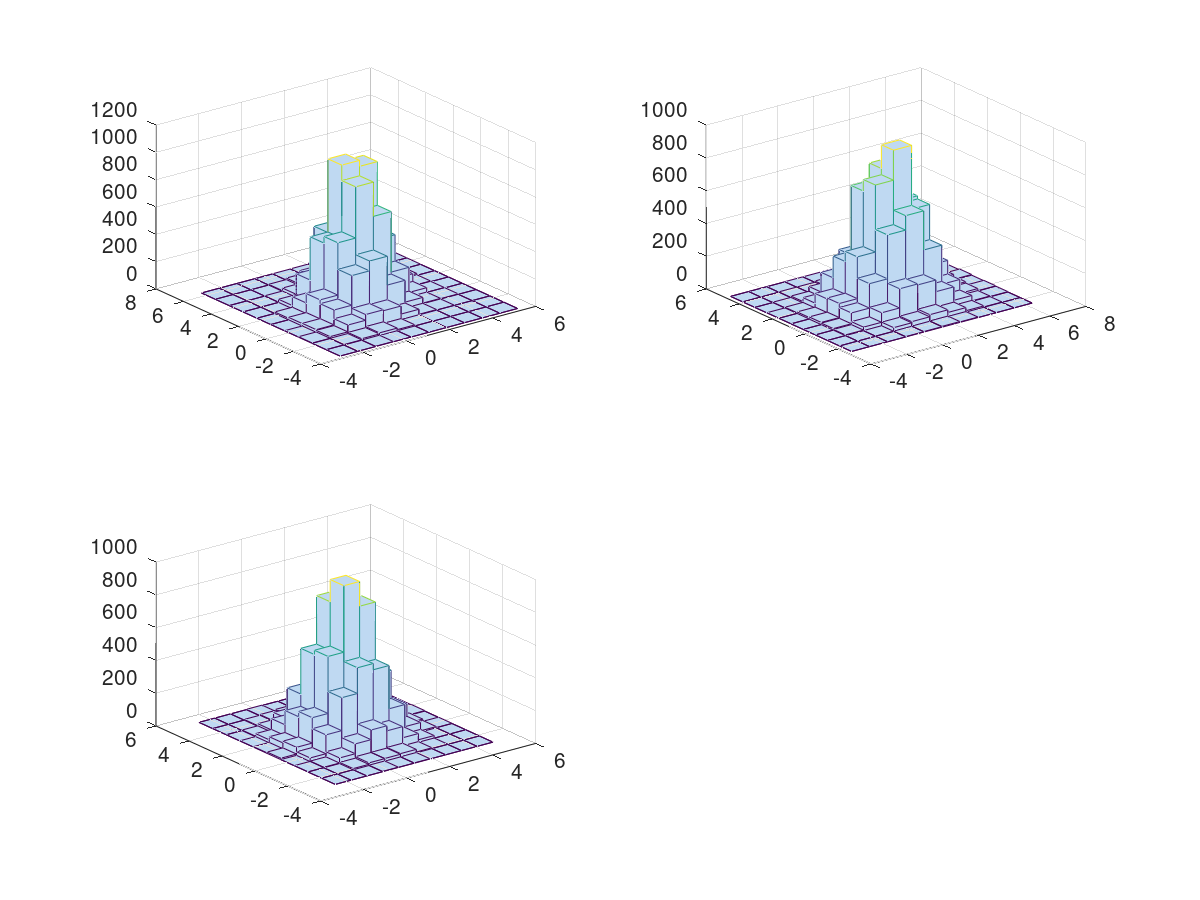
\includegraphics[scale=0.2]{t_0.2.png}
\\*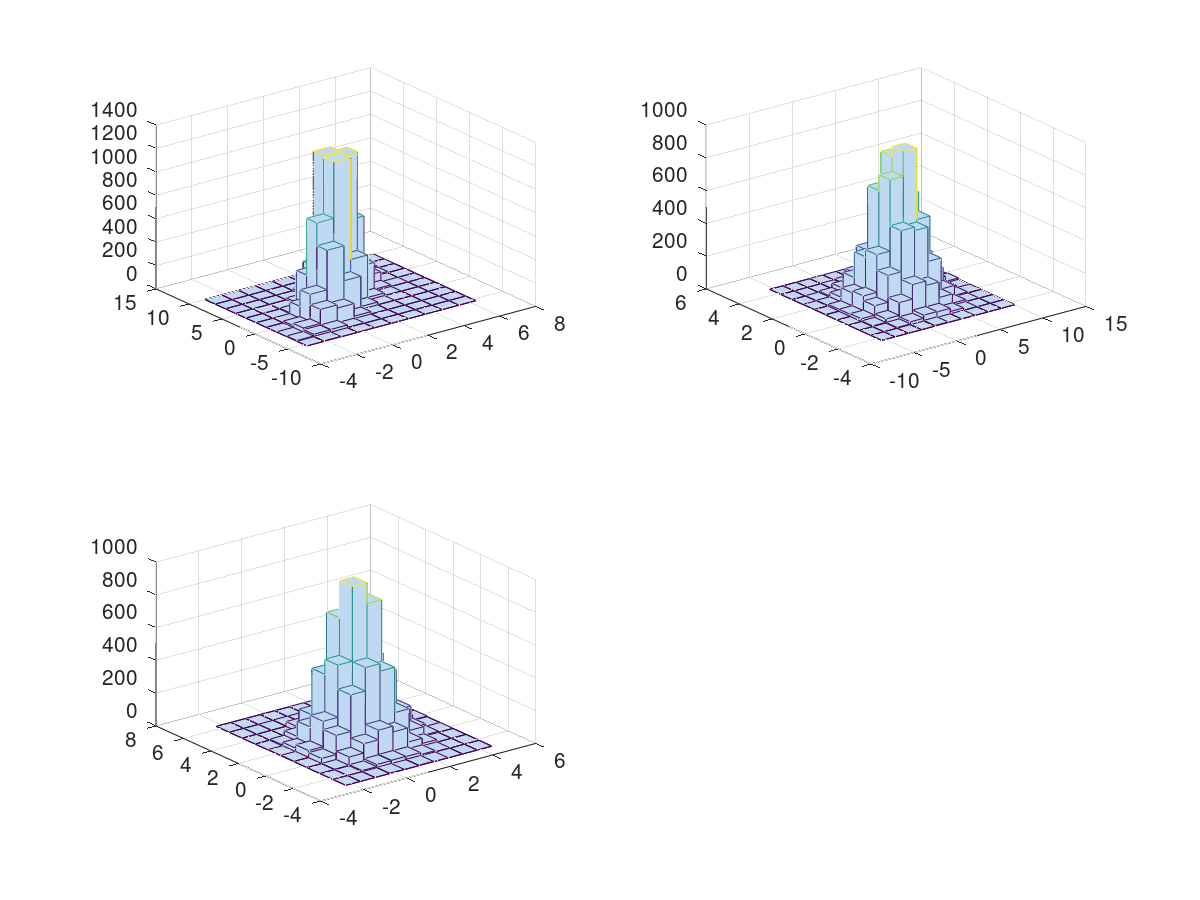
\includegraphics[scale=0.2]{t_0.5.png}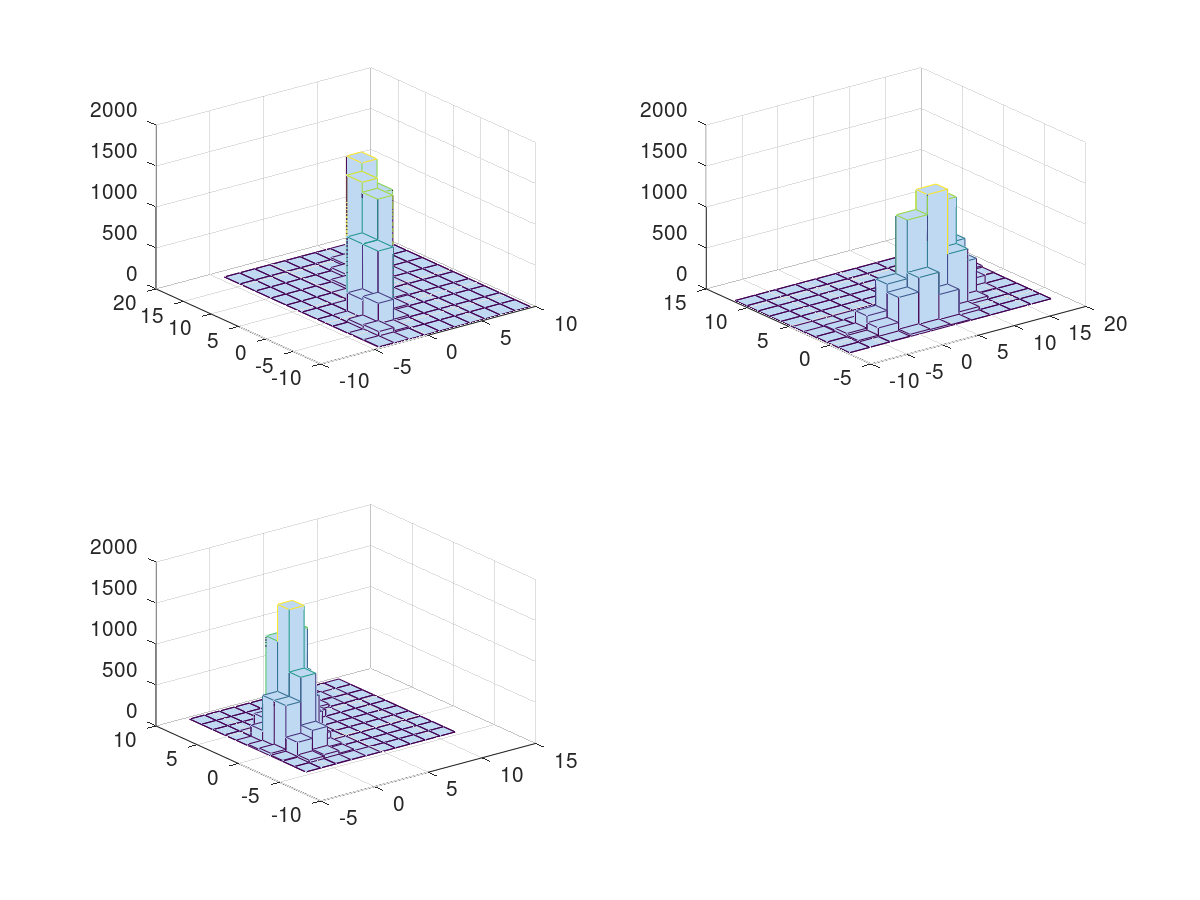
\includegraphics[scale=0.2]{t_1.0.png}
For the individul values, mean with mean+3*std,mean-3*std are plotted in the below figure.
\\*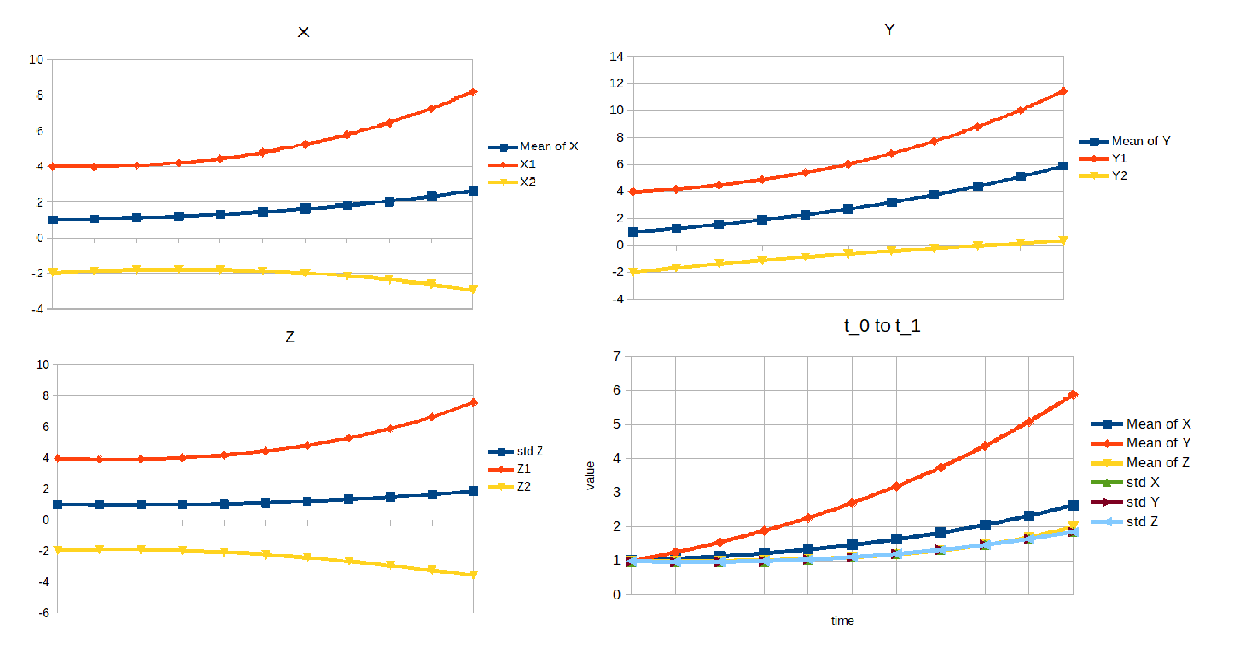
\includegraphics[scale=.5]{x-y-z.png}

$\textbf{Comments}$: 
\\*It is observed that initial noise or variation in the data is increased with time. We can extend this model to solve variety of problems to qantify uncertainity in the predicted output, especially in IVPs where characterizaing initial condition is difficult.
\\*If we run the simulation using (1,1,1) as we defined in the beginning, at t=1 (x,y,z)=(2.66,6.04,1.62) which is closer to the mean values that we got using monte carlo.






\end{document}
